\section*{Recurrent Neural Networks}
\color{black}
\subsection*{Simple RNNs}
Given a non-i.i.d. sequence $\mathbf x^1,...,\mathbf x^T$ derive a sequence of states $z^1, ..., z^T$ according to the Markovian time-invariant update $z^t = F_\theta(z^{t-1}, x^t)$. Produce an output sequence via $\mathbf y^t=H_\varphi(\mathbf z^t)$ (where $\mathbf y^T$ may be used for classification).

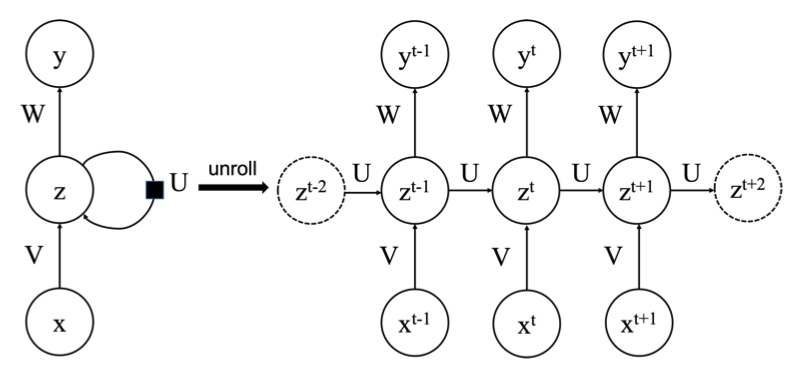
\includegraphics[width=.87\linewidth]{rnn_unrolled.png}

$F_\theta$ and $H_\varphi$ are parametrized as $F_{U,V}(\mathbf z, \mathbf x)=\phi(U\mathbf z+V\mathbf x)$ and $H_W(\mathbf z)=\psi(W\mathbf z)$ for activation functions $\phi, \psi$.
 
\textbf{Backpropagation (through time)}:

\resizebox{\linewidth}{!}{Propagation: $\color{teal}\frac{\partial z^{k+1}}{\partial z^{k}} \!=\! \frac{\partial \phi(U z^k + V x^{k+1})}{\partial z^{k}} \!=\! diag(\dot \phi(U z^k + V x^{k+1})) U$}

\hspace{47pt} $\color{blue}\frac{\partial y^s}{\partial z^s} = \frac{\partial \psi(W z^s)}{\partial z^{s}} = diag(\dot \psi(W z^s)) W$

Per State: $\color{violet}\frac{\partial E}{\partial z^q} = \sum_{s=q}^T \frac{\partial E}{\partial y^s} \frac{\partial y^s}{\partial z^q} = \sum_{s=q}^T \frac{\partial E}{\partial y^s} {\color{blue}\frac{\partial y^s}{\partial z^s}} \prod_{k=q}^{s-1} \color{teal}\frac{\partial z^{k+1}}{\partial z^k}$

$\bullet \frac{\partial E}{\partial W} = \sum_{s=1}^T \frac{\partial E}{\partial y^s} \frac{\partial y^s}{\partial W} = \sum_{s=1}^T (\Dot{\psi}(Wz^s) \odot z^s) \frac{\partial E}{\partial y^s}$

$\bullet \frac{\partial E}{\partial U} \!=\! \sum_{q=1}^T {\color{violet}\frac{\partial E}{\partial z^q}} \frac{\partial z^q}{\partial U} \!=\! \sum_{q=1}^T (\dot\phi(Uz^{q\text{-}1}+Vx^{q}) \odot z^{q\text{-}1}) {\color{violet}\frac{\partial E}{\partial z^q}}$

$\bullet \frac{\partial E}{\partial V} \!=\! \sum_{q=1}^T {\color{violet}\frac{\partial E}{\partial z^q}} \frac{\partial z^q}{\partial V} \!=\! \sum_{q=1}^T (\dot\phi(Uz^{q\text{-}1}+Vx^{q}) \odot x^{q}) {\color{violet}\frac{\partial E}{\partial z^q}}$
\\

$\bullet \color{purple}\frac{\partial E}{\partial \theta} = \sum_{t=1}^T \!\!\frac{\partial E}{\partial y_t} \frac{\partial y_t}{\partial z_t} \sum_{i=1}^t\!( \prod_{k=t}^{i+1} \!\frac{\partial z_k}{\partial z_{k-1}}) \frac{\partial F_\theta(z,x)}{\partial \theta} \big\vert_{z=z^{i-1}\!\!, x = x^{i-1}}$

\textbf{Exploding/Vanishing Gradients}:\\ 
$\norm{A}_2=\max_{x:\norm{x}=1}\norm{Ax}_2=\sigma_1(A) \hfill \norm{AB}_2\leq \norm{A}_2\norm{B}_2$\\
In backpropagation the following derivative occurs:\\
$\frac{\partial z^T}{\partial z^0}=\dot{\Phi}^TU\cdots \dot{\Phi}^1U$ where $\dot{\Phi}^t=\text{diag}(\dot \phi (Uz^{t-1}+Vx^t))$ and $\exists \alpha : $ $\dot{\Phi}^t\leq\alpha I$ (RELU: $\alpha=1$, Sigmoid: $\alpha=1/4$). If $\sigma_1(U)<1/\alpha$, $\norm{\frac{\partial z^T}{\partial z^0}}_2\leq (\alpha\sigma_1(U))^T\rightarrow 0$ as $T\rightarrow \infty $ giving vanishing gradients. Similarly, exploding gradients occur.

\textbf{Bi-Directional RNN}:\\
Additionally evolve $\Tilde{z}^t=\phi(\Tilde{U}\Tilde{z}^{t+1}+\Tilde{V}x^t)$ with $\Tilde{z}^{T+1}=0$. Modified output map couples the two: $y^t=\psi(Wz^t+\Tilde{W}\Tilde{z}^t)$.

\textbf{Deep RNN/Stacked RNN/Hierarchical RNN:}\\ 
$z^{t,l}=\phi(U^lz^{t-1,l}+V^lz^{t,l-1})$ where $l$ denotes the layer and $z^{t,0}=x^t$. Output computed from last state $y^t=\psi(Wz^{t,L})$.

\subsection*{Gated Memory Units}
\textit{Addressing the problem of vanishing/exploding gradients}\\
Gating unit: $z_{gated} =\sigma(G\zeta)\odot z$ where $\sigma(\cdot) \in [0,1]$. Gating units are embedded into gated units (LSTMs or GRUs).\\

\textit{We neglect bias terms in the following.}\\
\textbf{Long-Short-Term-Memory Unit (LSTM) - 3 Gates}\\
\begin{minipage}{0.5\linewidth}
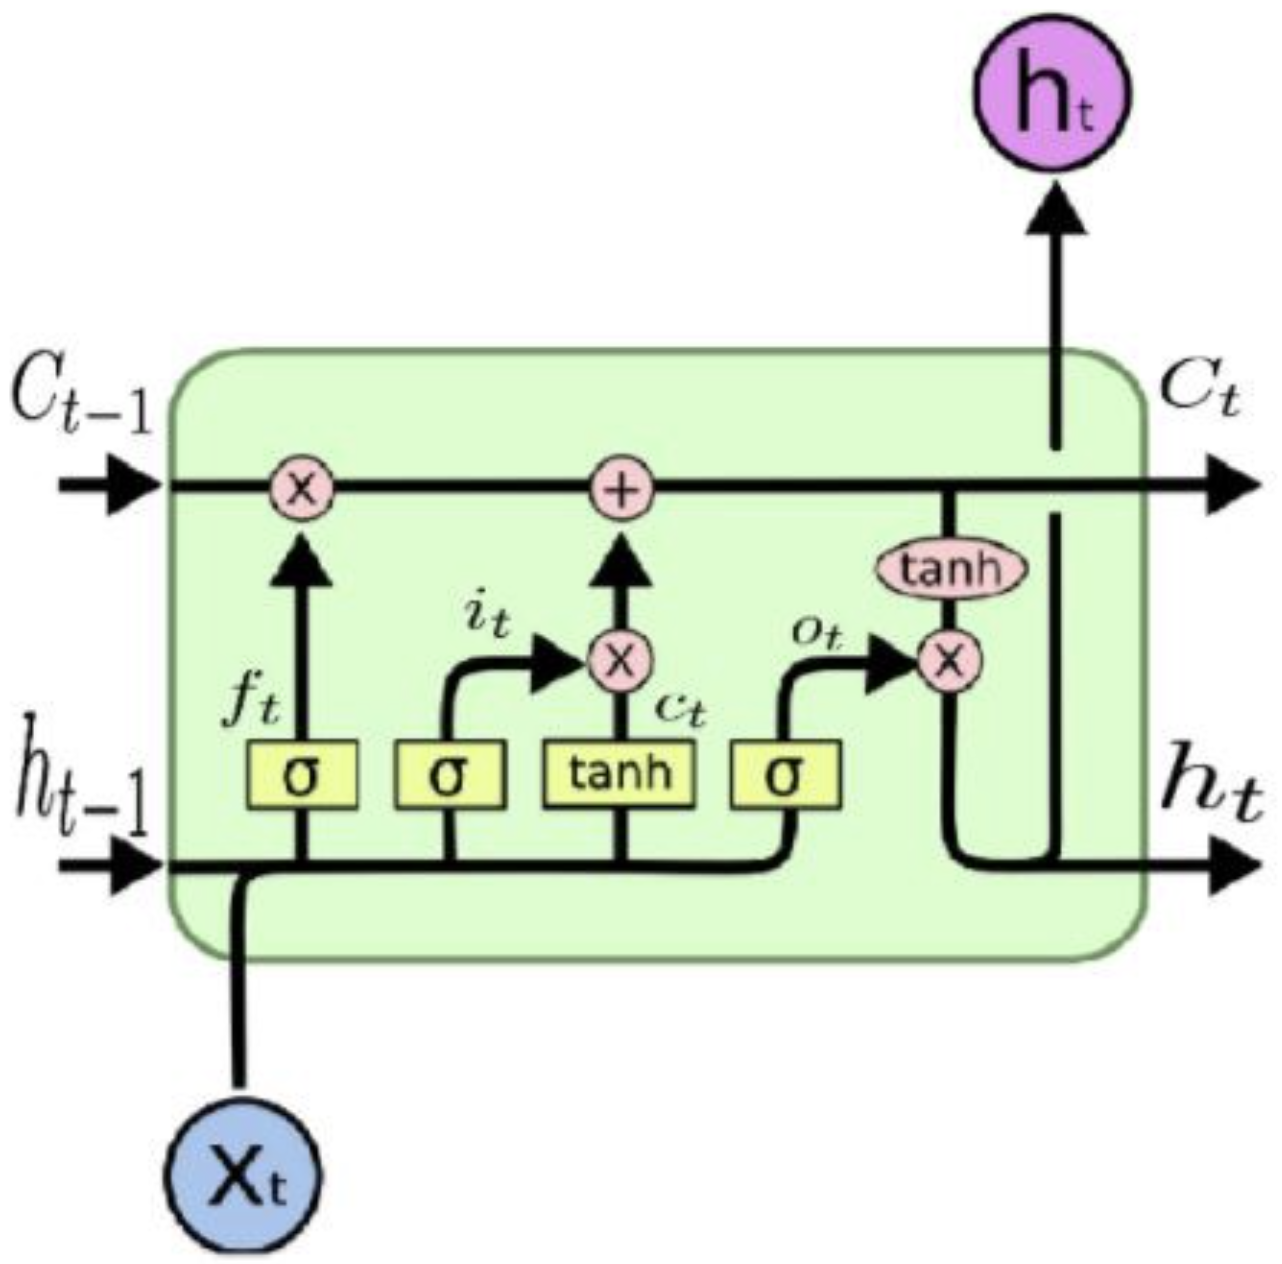
\includegraphics[width=\linewidth]{lstm_cell.png}
\end{minipage}
\begin{minipage}{0.5\linewidth}
    Augmented Input:\\
    $\tilde{x}_t = [h_{t-1}, x_t]$\\

    Output Gate:\\
    $h_{t} = \sigma(H \tilde{x}_{t}) \otimes \tanh(U C_{t})$\\
    
    Forget \& Input Gate:\\
    $C_t = \sigma(F \tilde{x}_t) \odot C_{t-1}$
    
    \hspace{8pt} $+\ \sigma(G \tilde{x}_t) \odot \tanh(V \tilde{x}_t)$\\

    Output Processing:\\
    $y_t = W h_t$
\end{minipage}
\underline{3} gating weight matrices: $H, F, G$, \underline{2} propagation weight matrices $U,V$, and \underline{1} output weight matrix $W$. \underline{6} in total. \\
\textbf{Gated Recurrent Unit (GRU) - 2 Gates}\\
\textit{Introduced to simplify LSTMs (less gates, less weights). The forget gate and input gate are convexly combined and the context cell/hidden state duality is removed.}\\

\begin{minipage}{0.5\linewidth}
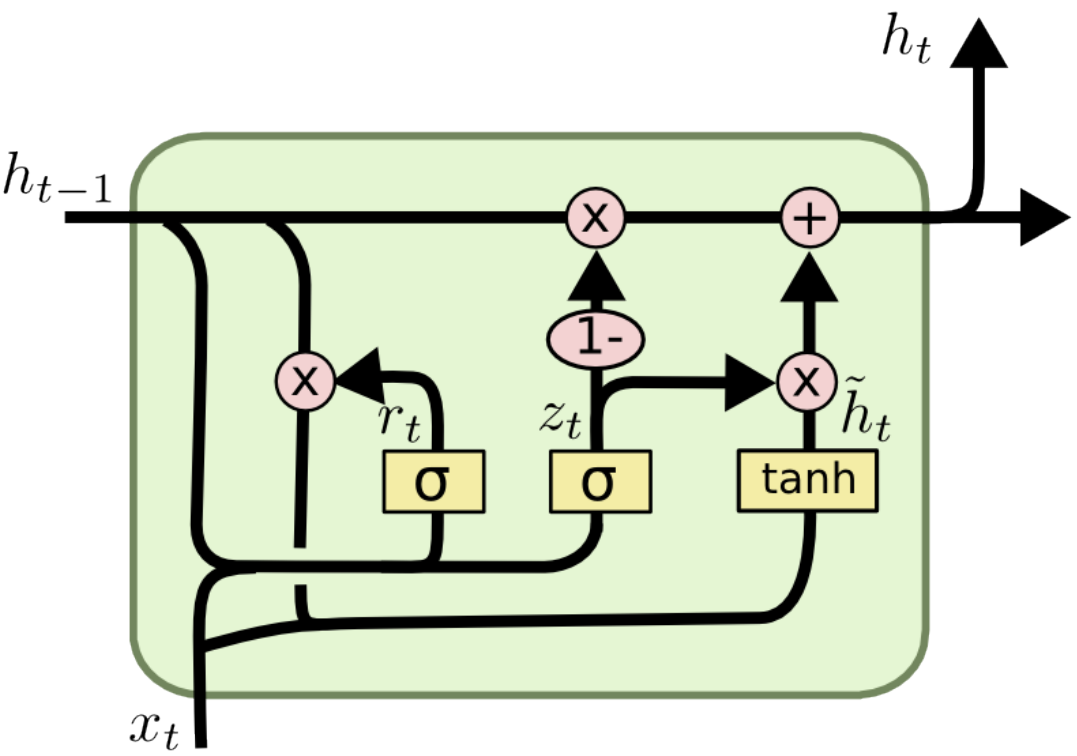
\includegraphics[width=\linewidth]{gru.png}
\end{minipage}
\begin{minipage}{0.5\linewidth}
Reset Gate:\\
$r_t = \sigma(H [h_{t-1}, x_t])$\\[-2pt]

Proposed Input:\\
$\tilde{h}_t = \tanh(V[r_t \odot h_{t-1}, x_t])$\\[-2pt]

Update Gate (Forget\&Input):\\
\resizebox{\linewidth}{!}{$h_t = (1\text{-}\sigma(G[h_{t\text{-}1}, x_{t\text{-}1}])) \odot h_{t\text{-}1}$}

\hspace{7pt} $+\ \sigma(G[h_{t\text{-}1}, x_{t\text{-}1}]) \odot \tilde h_t$\\[-2pt]

Output Processing\\ $y_t = W h_t$
\end{minipage}
\underline{2} gating weight matrices: $H, G$, \underline{1} propagation weight matrix $V$, and $1$ output weight matrix $W$. \underline{4} in total.

\subsection*{Linear Recurrent (State-Space) Models}
Linear state space model: $z^{t+1}=Az^t+Bx^t$ with diagonalization $A=P\Lambda P^{-1}$ over $\mathbb{C}$. Change of basis leads to $\zeta^{t+1}=\Lambda\zeta^t+Cx^t$ with $\zeta^t=P^{-1}z^t$ in complex state space ($\max_j\abs{\lambda_j}\leq 1$ for stabilization). To ensure high representational power of these systems, we give enough modelling power to the output map $y^t=\text{MLP}(\text{Re}(G\zeta^t))$.

\subsection*{Causal ($y^t \perp x^s\ \forall s > t$) Seq2Seq Modelling via RNN}
To learn $p(\mathbf y^{1:T}\mid \mathbf x^{1:T})\approx \prod_{t=1}^Tp(\mathbf y^t\mid \mathbf x^{1:t}, \mathbf y^{1:t-1})$ parametrize $p(y^t | x^{1:t}, y^{1:t-1})$ through $x^{1:t} \overset{F}{\mapsto} z^t \overset{H}{\mapsto} \mu^t \mapsto p_{\mu^t}(y^t)$. By introducing feedback links from $y^{t-1} \to z^t$ we can ensure that $z^t$ incorporates all knowledge on $x^{1:t}, y^{1:t-1}$.

\textbf{Teacher Forcing:}\\
\underline{During training}, compute loss on predicted output but feed back in actual output. \\
\underline{During prediction}, feed back predicted outputs. Improves learning BUT gives exposure bias (model only learns step predictions). \\
\underline{Professor Forcing} is a variant of teacher forcing that randomizes whether to feed back in $y_{pred}$ or $y_{true}$.\\
\textbf{Encoder-Decoder Model:} \\[2pt]
Encoder: $(\mathbf x^1,...,\mathbf x^T)\mapsto \mathbf z, \quad \mathbf z=\mathbf z^T$ (RNN)\\
Decoder $\mathbf z\mapsto (\mathbf y^1,...,\mathbf y^S)$ (RNN with output feedback)
\newcolumn
